\begin{wrapfigure}{t!}{0.5\textwidth}
	%\begin{figure}
	\centering
	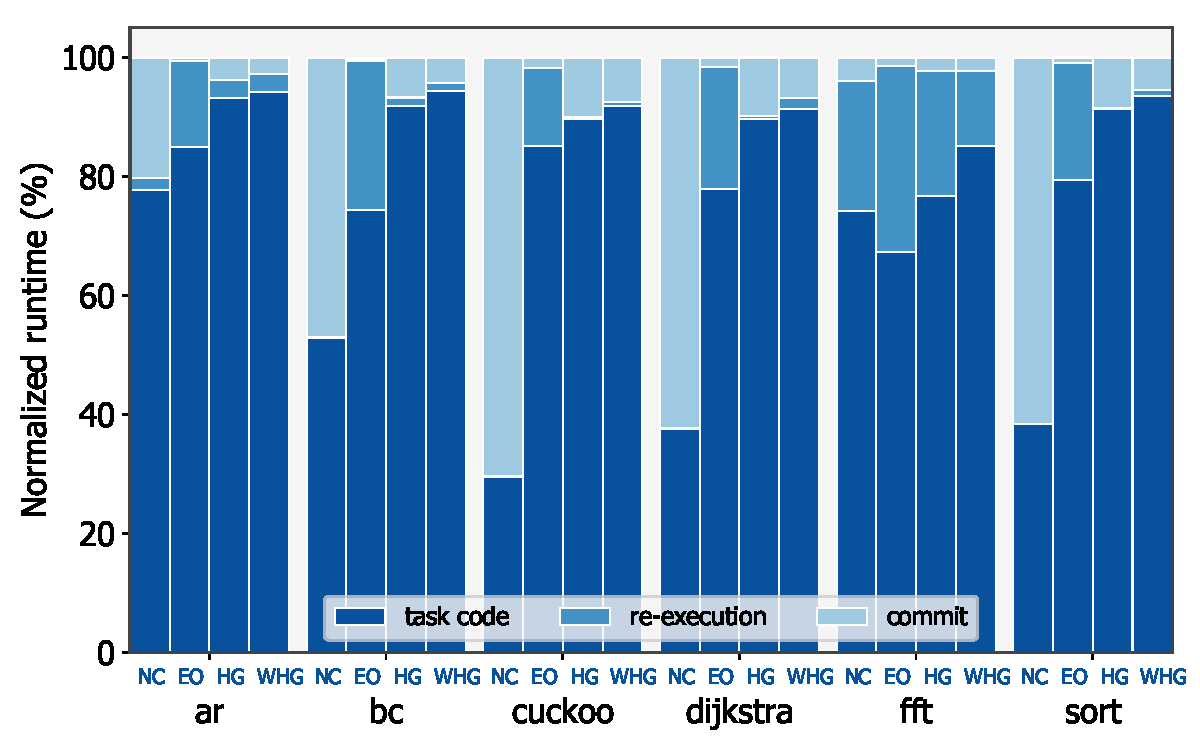
\includegraphics[width=0.5\columnwidth]{figures/coalEfficiency}
    \caption{Breakdown of overhead for the proposed coalescing strategies
relative to the baseline without coalescing.
NC: no coalescing, EO: energy-blind coalescing, HG: history-guided coalescing, WHG:
energy- and task-aware coalescing. All coalescing strategies reduce total
overhead and maximize useful work. HG and WHG perform better than EO.}
	\label{fig:overallOverheadBreakdown}
	%\end{figure}
\end{wrapfigure}

Our evaluation quantitavely demonstrates that \sys (i) \emph{reduces the memory
protection overhead} by coalescing, (ii) \emph{improves execution speed} for
conservative static task decompostions compared to state-of-the-art runtimes; %
and (iii) \emph{provides computation progress} at the sub-task granularity,
preventing non-termination at adverse energy conditions where state-of-the-art
runtimes fail. We measured the execution time of the benchmarks implemented
using \sys with each variant of the two proposed adaptation mechanisms:
\emph{task coalescing} and \emph{task downsizing}. We compared \sys's best
configurations against a state-of-the art system, Alpaca~\cite{alpaca}. We have
also broken down \sys's overhead to explain the source of \sys's improved
performance.

\subsection{Characterization of Overhead}
\label{sec:coala_overhead}

%\indent \textbf{Overhead Reduced by Coalescing.}

\subsubsection{Overhead Reduced by Coalescing}
\label{sec:overhead-coalescing}

For each coalescing strategy from Section~\ref{sec:task_adaptation} (EO, HG,
and WHG) and for a baseline without coalescing (NC), we have measured the time
spent on (i) executing useful task code, including \sys's overhead on access to
protected variables, (ii) re-executing task code after a power failure, and
(iii) committing state to non-volatile memory at the end of each (coalesced)
task.  In this experiment the WISP was 15\,cm away from the signal generator
antenna.
%
The page size was set to the best performing value (32~B for \textbf{bc} and
256~B pages for the rest) identified in detailed evaluation of paging in
Section~\ref{sec:results_memory_management}.

The overhead incurred by each coalescing strategy is broken down in
Figure~\ref{fig:overallOverheadBreakdown}. Without coalescing enabled (NC), the
re-execution penalty is smallest, because the amount of work that can happen
between commits and may have to be re-executed if interrupted is smallest when
work from multiple static tasks is not combined.
%
However, any gain from a reduced re-execution penalty is cancelled out by
the increased commit overhead that is incurred at the end of each static
task.
%
Across all benchmarks, all coalescing strategies reduce more commit overhead
than the re-execution overhead they add.
%
This net overhead reduction is greatest in HG and WHG strategies compared
to the EO strategy. We attribute this discrepancy to EO's slow adjustment
of the target task size without regard to execution history.
%
In the subsequent experiments, we focus on the better-performing HG and WHG
strategies.


\begin{figure}
	\centering
	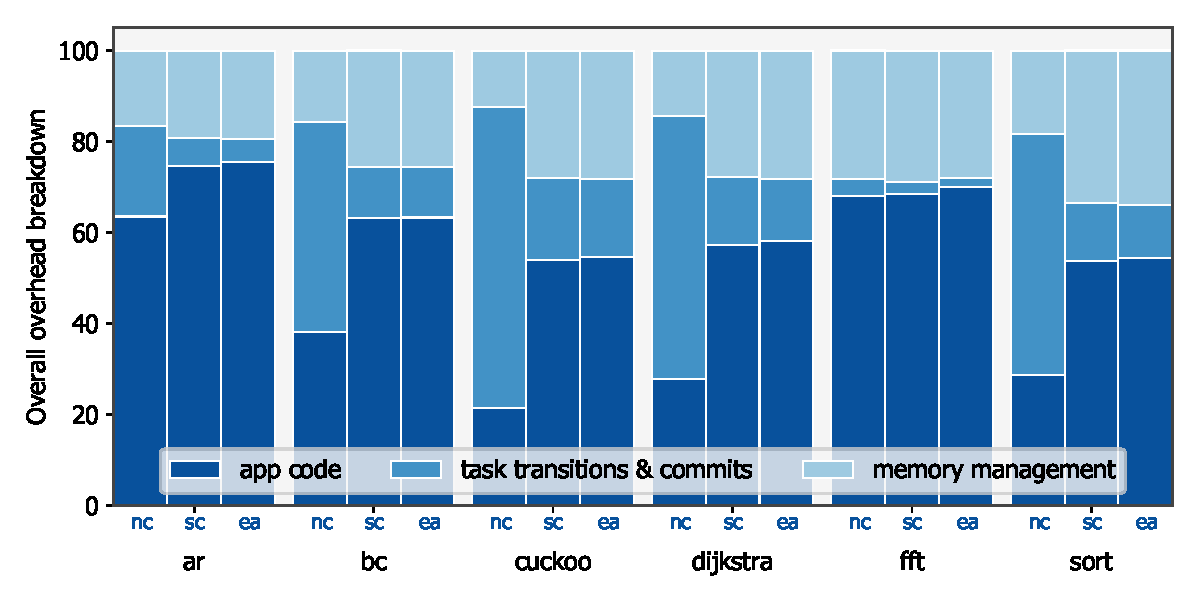
\includegraphics[width=0.49\columnwidth]{figures/overallOverhead}
	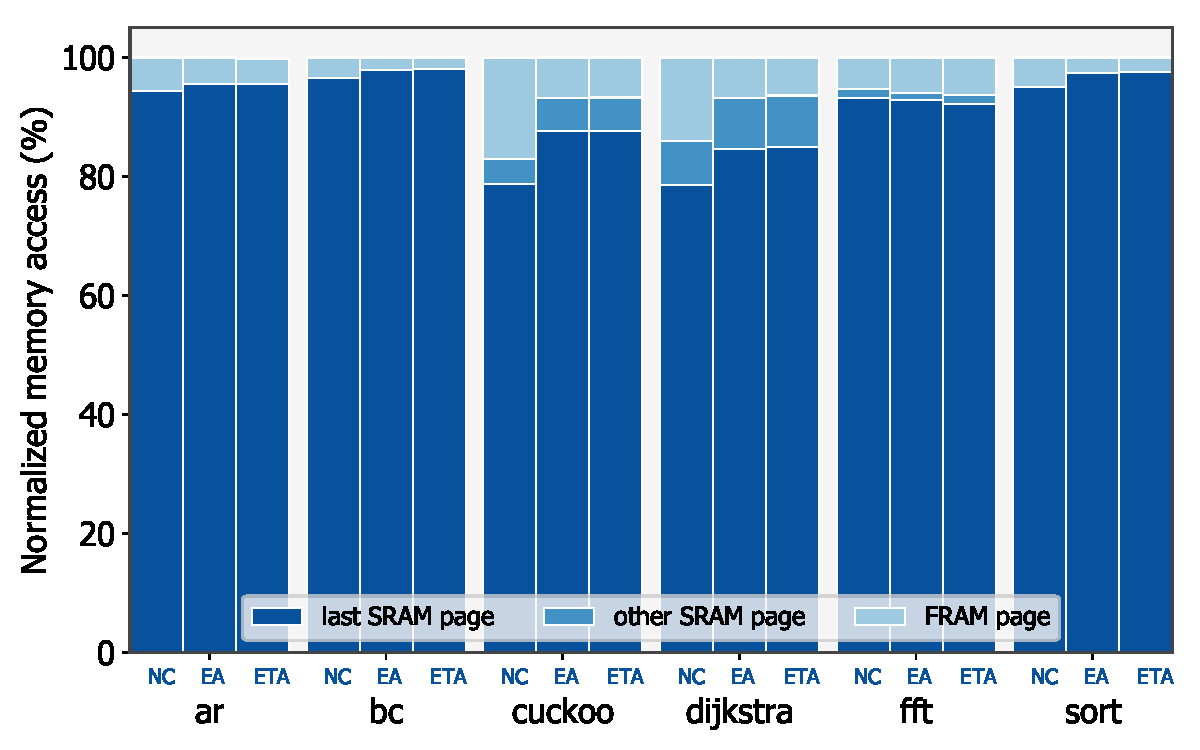
\includegraphics[width=0.49\columnwidth]{figures/memAccess}
	\caption{\sys kernel overhead: a breakdown of time spent in
the application and in the runtime (left) and a breakdown of protected memory
accesses into three types with different costs. NC: no coalescing, HG:
history-guided coalescing, WHG: weighted history-guided coalescing.}
	\label{fig:coalEfficiency}
\end{figure}

%\textbf{\sys Kernel Overhead Breakdown.}

\subsubsection{\sys Kernel Overhead Breakdown}

Figure~\ref{fig:coalEfficiency} (left) breaks down the time spent on executing
useful task code and committing further into time spent by the application and
time spent by \sys's runtime.
%
This dataset is generated in a separate experiment with the same setup as the
previous experiment in Section~\ref{sec:overhead-coalescing}.
%
Consistent with the previous results in
Figure~\ref{fig:overallOverheadBreakdown}, commit overhead is highest when
coalescing is not used to reduce the number of commits.
%
However, coalescing increases the cost of each access to a protected variable,
since work in the address translation in the paging system increases as the
task size grows.
%
For both coalescing strategies (HG and WHG) accesses to protected variables
constitute about 30\% of the runtime overhead. Dynamic address translation
necessary on each protected access is the most critical bottleneck for \sys.

%\textbf{Protected Memory Accesses Breakdown.}

\subsubsection{Protected Memory Accesses Breakdown}

Figure~\ref{fig:coalEfficiency} (right) breaks down protected memory accesses
into three categories.
%
Each type of protected access incurs a different amount of overhead: access to
the same page in SRAM as the previous access is cheapest, access to a different
SRAM page has a larger cost, and access to a page that needs to be swapped in
from FRAM into SRAM is most expensive.
%
The results in the figure show that the overwhelming majority of accesses are
of the cheapest kind, which motivated us to optimize this access type in our
implementation (cf. Section~\ref{sec:impl:paging}).
%
The search for the accessed page in the \texttt{\underline{working}} buffer,
will return immediately when the page is the most recently accessed page.
%
Only \textbf{cuckoo}, \textbf{dijkstra}, and \textbf{fft} have non-negligible
number of accesses to a different SRAM page, which is due to the larger working
set and a less regular access pattern in these applications.
%
In general, memory access patterns are shaped by the application, and the more
program state is protected, the higher the rate of page swaps.

\subsection{Execution time}
\label{sec:result_coalescing}

Having shown in Section~\ref{sec:coala_overhead} that coalescing reduces
overhead, we now investigate the outcome of this reduction on the total
execution time. We first investigate difference variants of \sys and
then compare the best variant to Alpaca.

%\textbf{\sys Speedup with Coalescing.}

\subsubsection{\sys Speedup with Coalescing}

Figure~\ref{fig:coalescing} shows the \sys run time with two coalescing
strategies (HG, WHG) normalized to the run time without coalescing (NC).
%
The experimental setup is the same as that in Section~\ref{sec:coala_overhead}.
%
The results in Figure~\ref{fig:coalescing} (left) show that all benchmarks
complete faster with coalescing than without coalescing: from 25\% faster
(\textbf{ar}) up to 70\% faster (\textbf{sort}).
%
This speedup is a consequence of the reduced overhead demonstrated in
Section~\ref{sec:coala_overhead}.
%
However, the magnitude of the speedup is (1) highly application-dependent and
(2) largely similar across the two coalescing strategies, with the exception of
\textbf{fft}.
%
In some cases (\textbf{bc}, \textbf{cuckoo}, \textbf{sort}) the history-guided
feature in the coalescing algorithm is counter-productive.
%
This occurs in task decompositions with a uniform task energy, where counting
tasks disregarding their energy provides an equal amount of information with a
smaller effort.
%
In \textbf{fft}, tasks are not uniform, and accounting for task energies is
beneficial. In fact, the lack of task energy awareness is detrimental: with HG
\textbf{fft} runs slower than without any coalescing (NC).
%
The speedup is highest for \textbf{bc}, \textbf{cuckoo}, \textbf{dijkstra} and
\textbf{sort}, because their tasks are small and are easily coalesced,
eliminating many unnecessary commits.

\begin{figure*}
	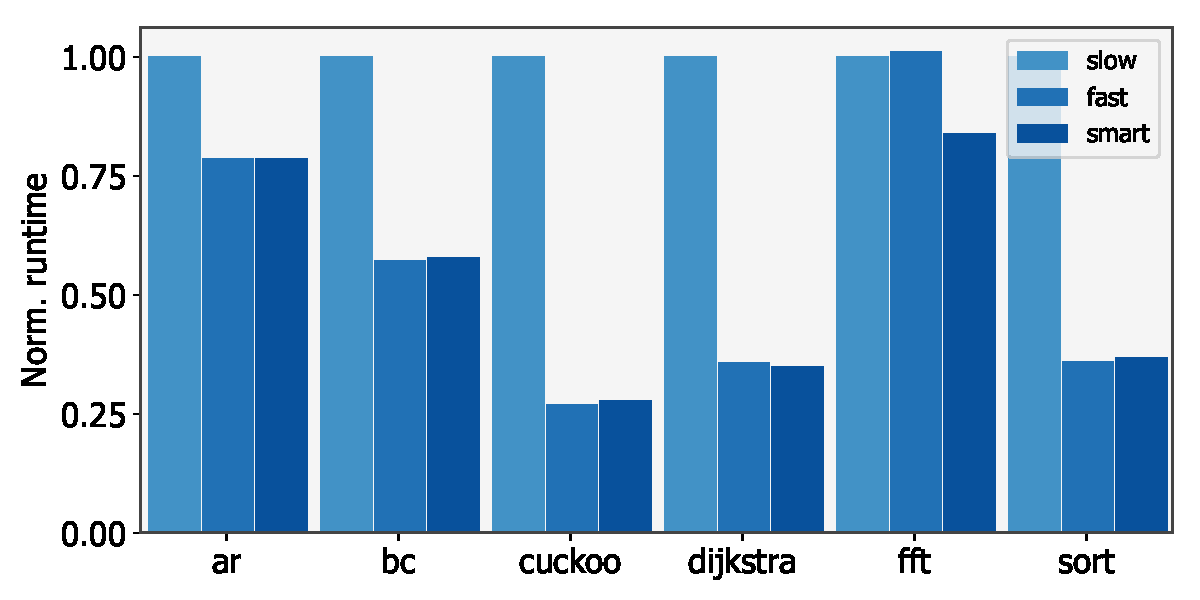
\includegraphics[width=0.5\columnwidth]{figures/coalStrategies}%
	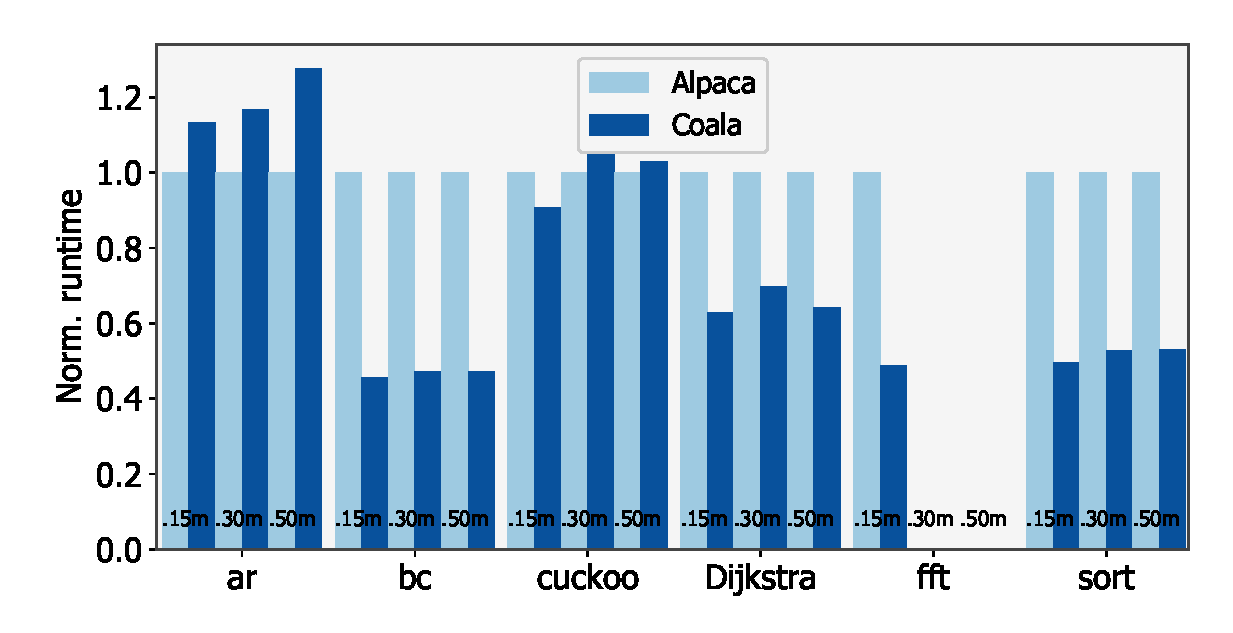
\includegraphics[width=0.5\columnwidth]{figures/coala_alpaca_gcc}
    \caption{\sys's coalescing performance. Left: Application execution time
with coalescing strategies (HG and WHG) normalized to the execution time
without coalescing. Right: Execution time with the WHG variant of \sys,
normalized to the execution time with Alpaca, as a function of distance to the
energy source.}
	\label{fig:coalescing}
	\label{fig:runtime}
\end{figure*}

%\begin{wrapfigure}{t!}{0.5\textwidth}
%	%\begin{figure}
%	\centering
%	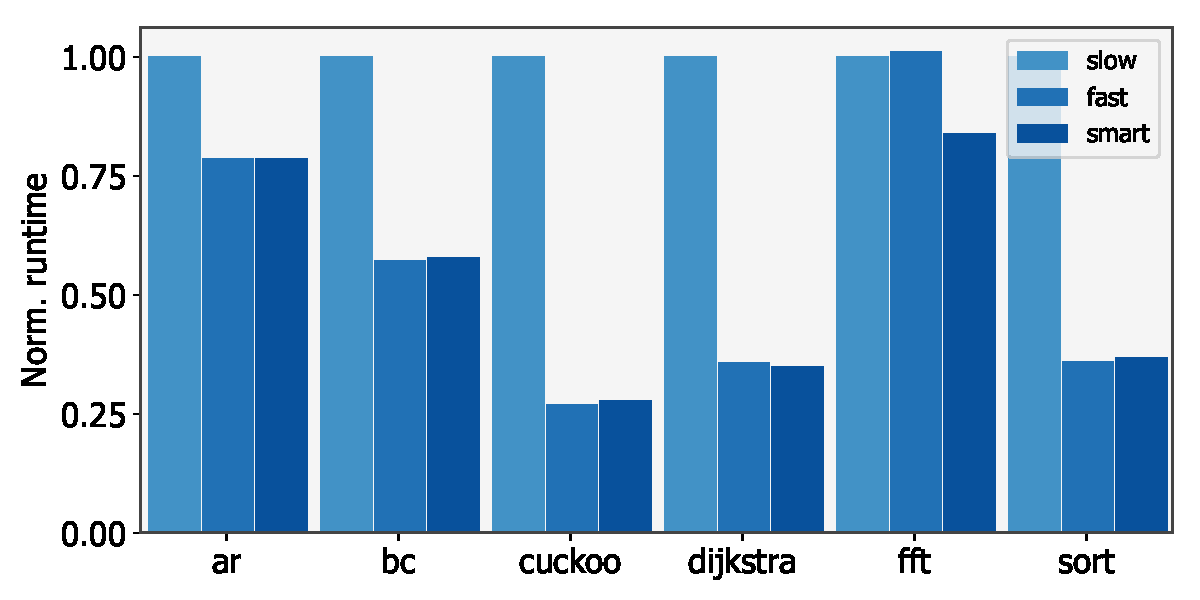
\includegraphics[width=0.5\columnwidth]{figures/coalStrategies}
%	\caption{Coalescing strategies (HG and WHG) run time per application on intermittent power (RF generator at 15\,cm from the WISP), compared to \sys without coalescing (NC). Coalescing provides significant improvements: from 0.25 (\textbf{ar}) up to 0.70 (\textbf{sort}) compared to a non-coalescing system.}
%	\label{fig:coalescing}
%	%\end{figure} 
%\end{wrapfigure}
%
%\begin{wrapfigure}{t!}{0.5\textwidth}
%	%\begin{figure}
%	\centering
%	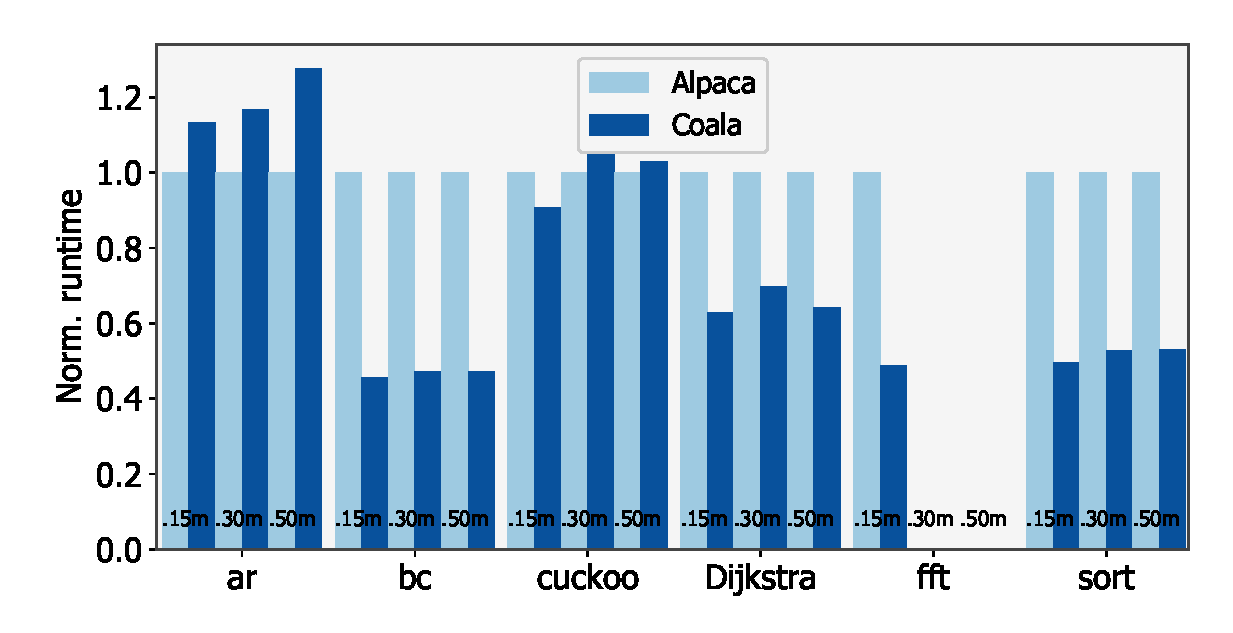
\includegraphics[width=0.5\columnwidth]{figures/coala_alpaca_gcc}
%    \caption{Application execution time with the WHG variant of \sys,
%normalized to the execution time with Alpaca, as a function of distance to the
%signal generator antenna. \sys outperforms Alpaca on the majority but not all
%of the benchmarks.}
%	\label{fig:runtime}
%%\end{figure}
%\end{wrapfigure}

%\textbf{Benefits of Adaptive Tasks.}

\subsubsection{Benefits of Adaptive Tasks}

We now compare \sys's performance to Alpaca~\cite{alpaca}---a
\emph{non-adaptive} task-based system with tasks fixed at compile time.
Figure~\ref{fig:runtime} (right) shows the average execution time of each
application for \sys and Alpaca, normalized to the latter. The results show
that \sys provides a performance benefit compared to Alpaca for most
applications, with the exception of \textbf{ar} and \textbf{cuckoo} at some
distances.  The speedup is greatest for applications with repeated write after
read dependencies throughout their code, particularly involving arrays
(\textbf{dijkstra}, \textbf{fft} and \textbf{sort}). \sys's virtualized memory
successfully amortizes the overhead of protecting memory that is accessed in
such patterns.  In applications without locality among accesses to protected
variables, including array elements, \sys incurs overhead from memory
virtualization that causes its performance to be comparable to (or worse than)
Alpaca (\textbf{ar}, \textbf{cuckoo}).

The \textbf{fft} benchmark did not complete at distances larger than
15\,cm~\footnote{At distances greater than 15~cm, energy incoming during
execution is negligible and stored energy is insufficient to complete some of
the static tasks.} with neither Alpaca, nor \sys \emph{without the downsizing
mechanism}. This is marked with $\infty$ signs in Figure~\ref{fig:coalescing}
(left).  This non-terminating condition cannot be avoided in Alpaca, due to the
fixed, non-adaptive nature of its tasks.  In contrast, our next experiment
shows how \sys's task downsizing adaptation mechanism eliminates this
non-termination, without changing the static tasks and without recompiling the
application.

In a separate experiment, we have enabled task downsizing in \sys and measured
the execution time for \textbf{fft} benchmark at 60\,cm from the signal
generator antenna --- even \emph{farther} than the distance at which this
benchmark failed to terminate in the previous experiment. \sys executed the
benchmark successfully without (NC) and with coalescing (WHG). The application
took longer to complete than at a shorter distance of 15~cm in the previous
experiment, because of smaller (negligible) incoming energy at the larger
distance. The variant without coalescing (NC) slowed down by 2.16$\times$ and the
variant with WHG coalescing slowed down by 2.31$\times$ slower, but at both
distances, WHG completed faster than NC.
%
For comparison, the run time with Alpaca is effectively infinite at this
distance, which is a consequence of its non-adaptive static tasks.


	

\subsection{Virtual Memory Performance}
\label{sec:results_memory_management}

We characterize the performance of \sys's virtual memory sub-system in an
experiment on a continuously-powered evaluation board described in
Section~\ref{sec:methodology}.  Figure~\ref{fig:page_size} quantifies the
effects of page size.

%\textbf{Effect of Page Size on Runtime.}

\begin{figure}
	\centering
	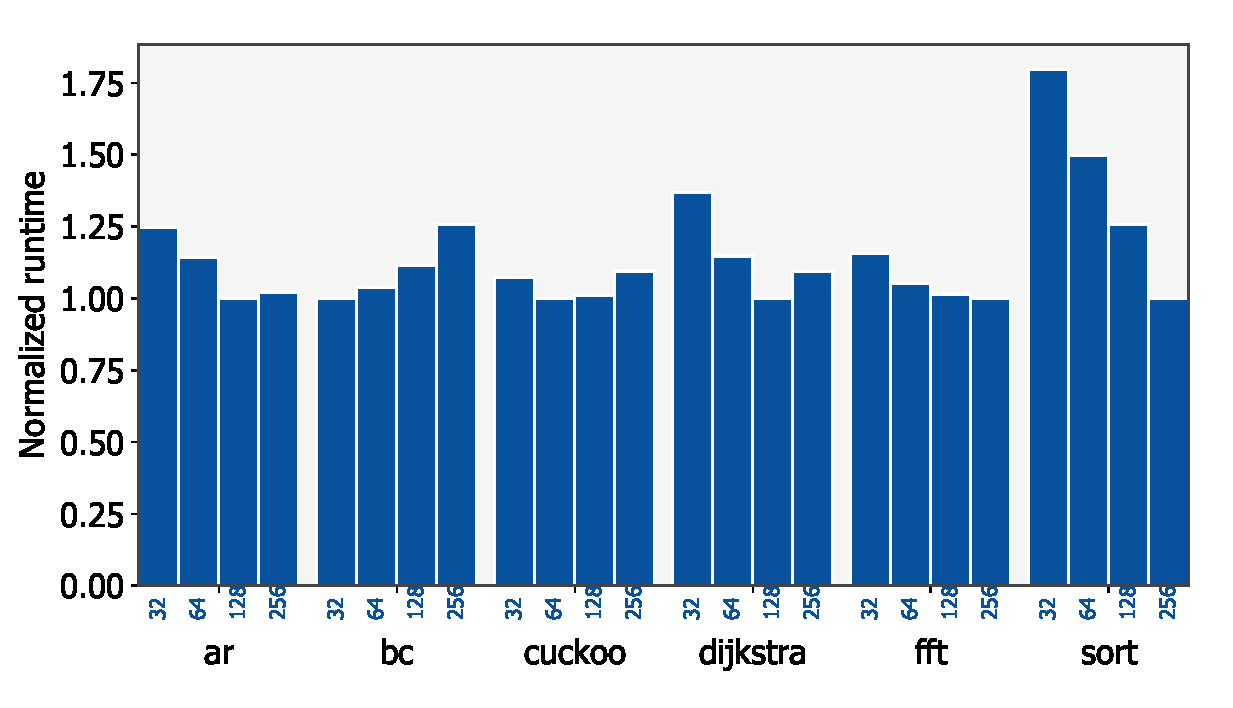
\includegraphics[width=0.49\columnwidth]{figures/page_exec-time}
	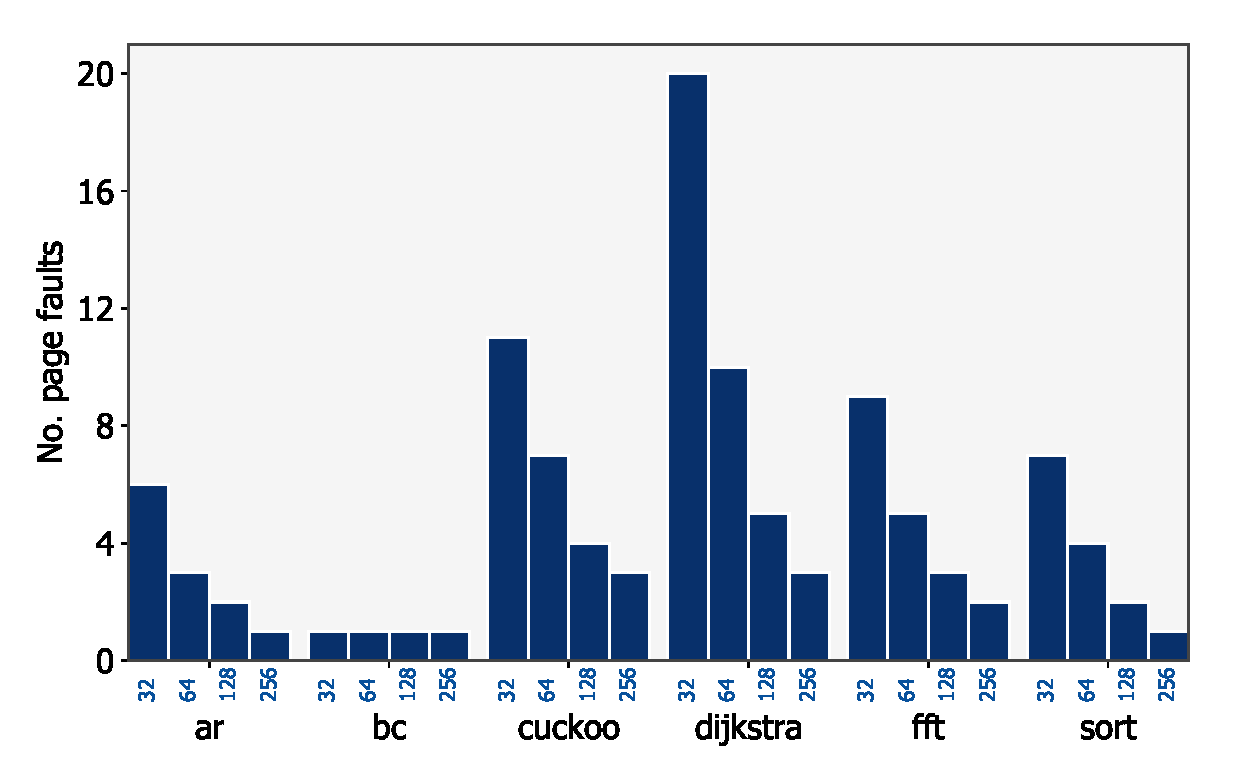
\includegraphics[width=0.49\columnwidth]{figures/pagePulls}
    \caption{Effect of page size on execution time (left) and on the number of
page faults (right). The execution time is normalized to the lowest in each set
of page sizes.}
	\label{fig:page_size}
\end{figure}


\subsubsection{Effect of Page Size on Runtime}

Figure~\ref{fig:page_size} (left) shows the execution time as a function
of page size, normalized to the lowest per-application performance among the
set of page sizes.
%
With some exceptions, a ``bathtub curve'' can be observed in the data.  For
some applications one of the two edges of the bathtub shape is missing, because
we did not evaluate a sufficiently wide range of page sizes.
%
The right edge of the bathtub is a consequence of the time spent copying
unnecessary data along with data of interest, because copies are at page
granularity.
%
The left edge of the bathtub is due to the overhead of swapping pages in
upon access.
%
The swap-in overhead is proportional to the number of page faults.
%
Page faults are more likely with smaller pages, as visible in the plot on the
right in Figure~\ref{fig:page_size}.
%
The data suggest that there is a page size, distinct from the largest or
smallest, that minimizes execution time. The best page size is not the same for
each application. Nevertheless, if a choice must be made for all applications,
128\,B pages perform well for most of them.

%\textbf{Effect of Page Size on Page Faults.}

\subsubsection{Effect of Page Size on Page Faults}

Figure~\ref{fig:page_size} (right) shows the number of page faults as a
function of page size.
%
The smaller the page the more likely that a memory access will land
outside that page and that a new page will need to be swapped in.
%
This trend is visible for all applications, exception \textbf{bc}. The total
amount of data accessed by \textbf{bc}, as well as its working set, is small.
Even with the smallest page, all accesses are contained within that page, and
no page faults occur. Without any page faults to begin with, increasing the
page size has no effect.

%\subsection{\sys Memory Footprint?}
%\label{sec:results_program_characterization}
%
%\begin{table}
%	\begin{tabular}{| c | c | c | c | c |}
%		\hline
%		\multirow{2}{*}{Application} & \multicolumn{2}{ c |}{Memory footprint} & \multirow{2}{*}{No. tasks} & \multirow{2}{*}{SLOC} \\
%		\cline{2-3}
%		{} & \sys & Alpaca & {} & {} \\
%		\hline\hline
%				\textbf{ar} & --- & --- & --- & ---\\
%		\hline
%				\textbf{bc} & --- & --- & --- & ---\\
%		\hline
%				\textbf{cuckoo} & --- & --- & --- & ---\\
%		\hline
%				\textbf{dijkstra} & --- & --- & --- & ---\\
%		\hline
%				\textbf{fft} & --- & --- & --- & ---\\
%		\hline
%				\textbf{sort} & --- & --- & --- & ---\\
%		\hline
%	\end{tabular}
%		\caption{Comparison between \sys and Alpaca benchmarks.}
%		\label{table:compiler_result}\vspace{-0.5cm}
%\end{table}

%\begin{table}[t]
%	\centering
%	\renewcommand{\tabcolsep}{1pt}
%	\begin{tabular}{|l|cc|cc|cc|cc|c|}
%		\hline
%		{} & \multicolumn{2}{c|}{{\bf Prot. bytes}} & \multicolumn{2}{c|}{{\bf \# Tasks}} & \multicolumn{2}{c|}{{\bf \# Prot. acc.}} & \multicolumn{2}{c|}{\bf SLOC} & {\bf Comp.} \\
%		App & Man. & Comp. & Man. & Comp. & Man. & Comp. & \multicolumn{1}{l}{\sys} & \multicolumn{1}{r|}{Chain~\cite{chain}} & {\bf time} \\
%		\hline\hline
%		bc & 22 & 22 & 10 & 15 & 81 & 93 & 351 &588 & 3\\
%		cem & 3492 & 3242 & 12 & 9 & 92 & 123 & 388 &721 & 2\\
%		cuckoo & 282 & 288 & 15 & 6 & 90 & 76 & 483 &762 & 6\\
%		rsa & 332 & 250 & 20 & 27 & 130 & 296 & 887 &1233 & 86\\
%		ar & 166 & 218 & 11 & 6 & 112 & 333 & 483 &762 & 34\\
%		sort & 104 & 104 & 4 & 2 & 70 & 23 & 180 & 287 & $<$1\\
%		dft$^\dagger$ & --- & --- & --- & --- & --- & --- & 222 & 293 & ---\\
%		%dd &  &  &  &  &  &  &  & 287 &  \\
%		\hline
%	\end{tabular}
%		\caption{Comparison between \sys and Alpaca benchmarks.}
%		\label{table:compiler_result}\vspace{-0.5cm}
%\end{table}
